\documentclass[13pt, t]{beamer}
% Presento style file
\usepackage{config/presento}

% custom command and packages
% custom packages
\usepackage{textpos}
\setlength{\TPHorizModule}{1cm}
\setlength{\TPVertModule}{1cm}

\newcommand\crule[1][black]{\textcolor{#1}{\rule{2cm}{2cm}}}



\usepackage{color, colortbl}

\title{\Large \hspace{-0.5cm} Andi Zilo: Collecting LexCauc List}
\author[shortname]{George Moroz}
\institute[shortinst]{Linguistic Convergence Laboratory, NRU HSE, Moscow, Russia}
\date{\begin{center} 
6 June 2019 \bigskip \\ 
Jena, LexCauc Workshop
\end{center}}

\begin{document}

\begin{frame}[plain]
\maketitle
\end{frame}
\begin{frame}{I collected the list! Hurrah!}
\pause
\begin{itemize}
\item 1500 from 1966 rows are filled (43 optional) 
\item 466 rows are not filled (41 optional) 
\begin{itemize}
\item 220 rows contain \textit{\_ipfv} (6 optional)
\end{itemize}
\item 5427 MB, \textbf{\LARGE 9 hours 13 minutes}
\end{itemize}
\end{frame}

\begin{frame}{So our main problems are...}
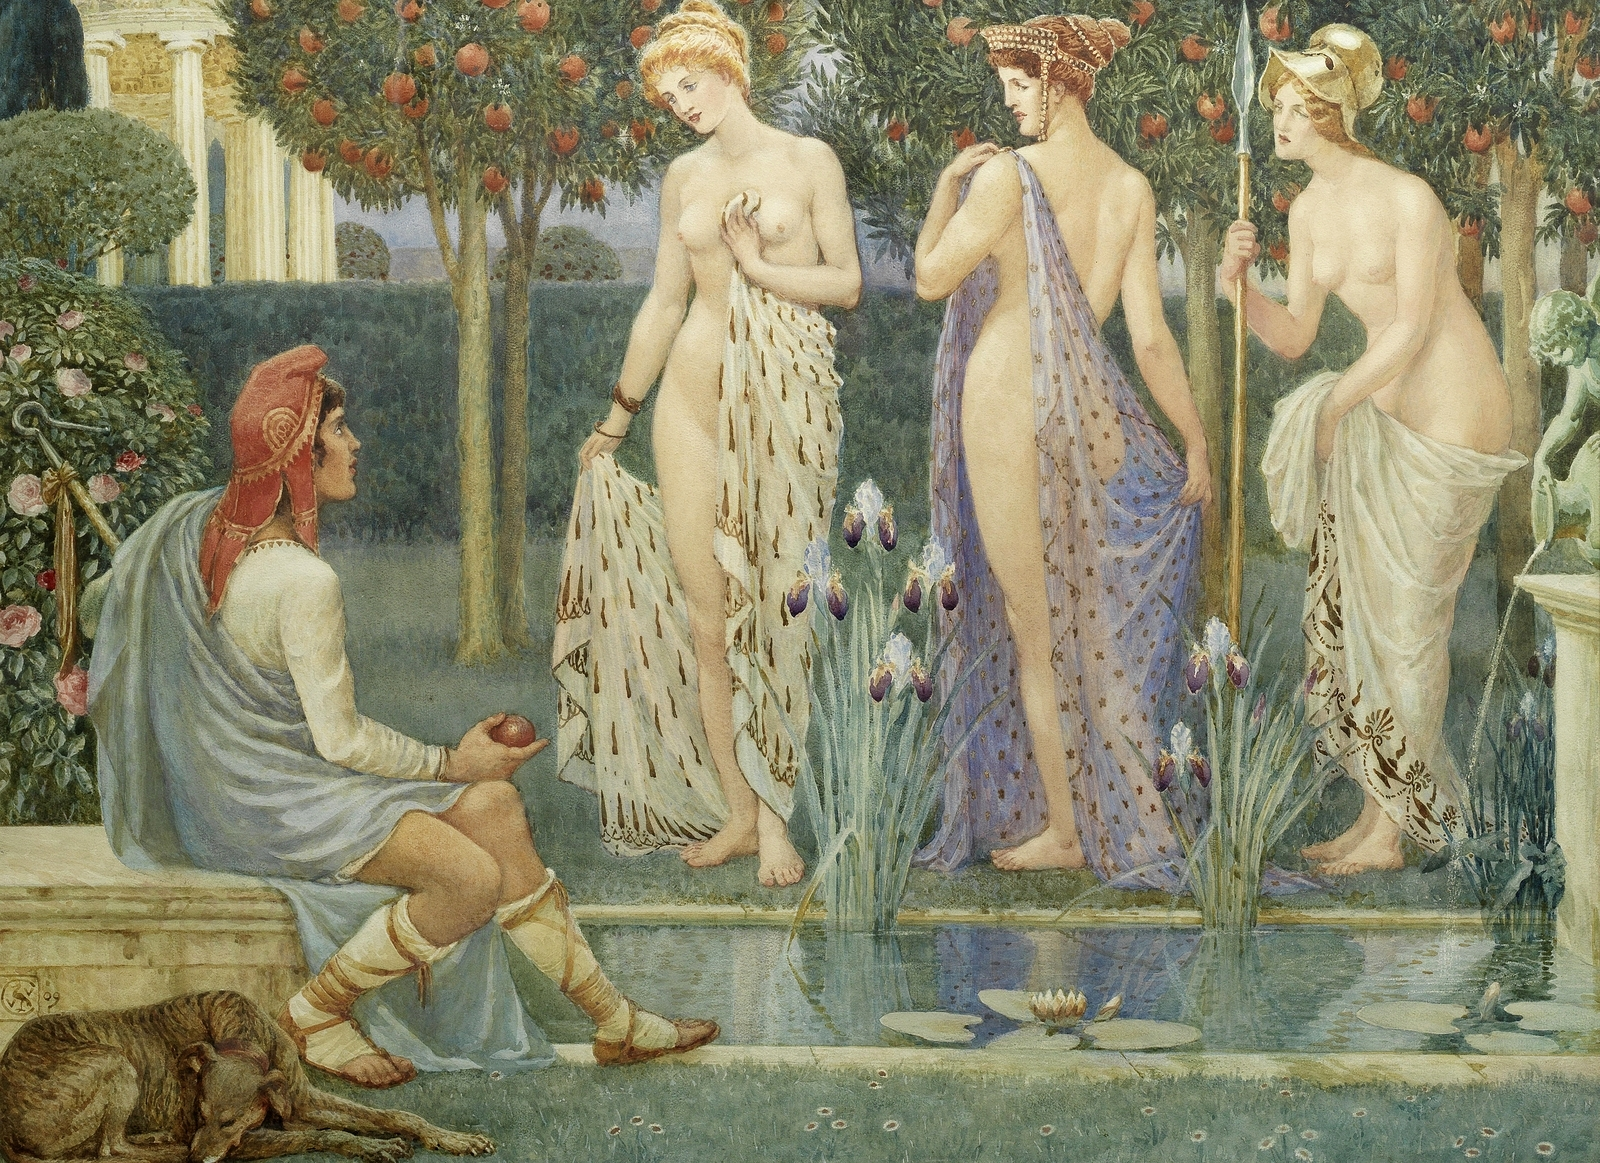
\includegraphics[height = 0.38\linewidth]{images/01_paris}
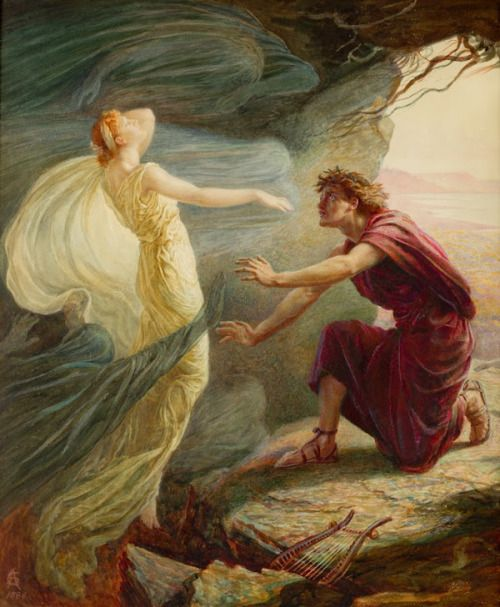
\includegraphics[height= 0.38\linewidth]{images/03_orpheus}\\
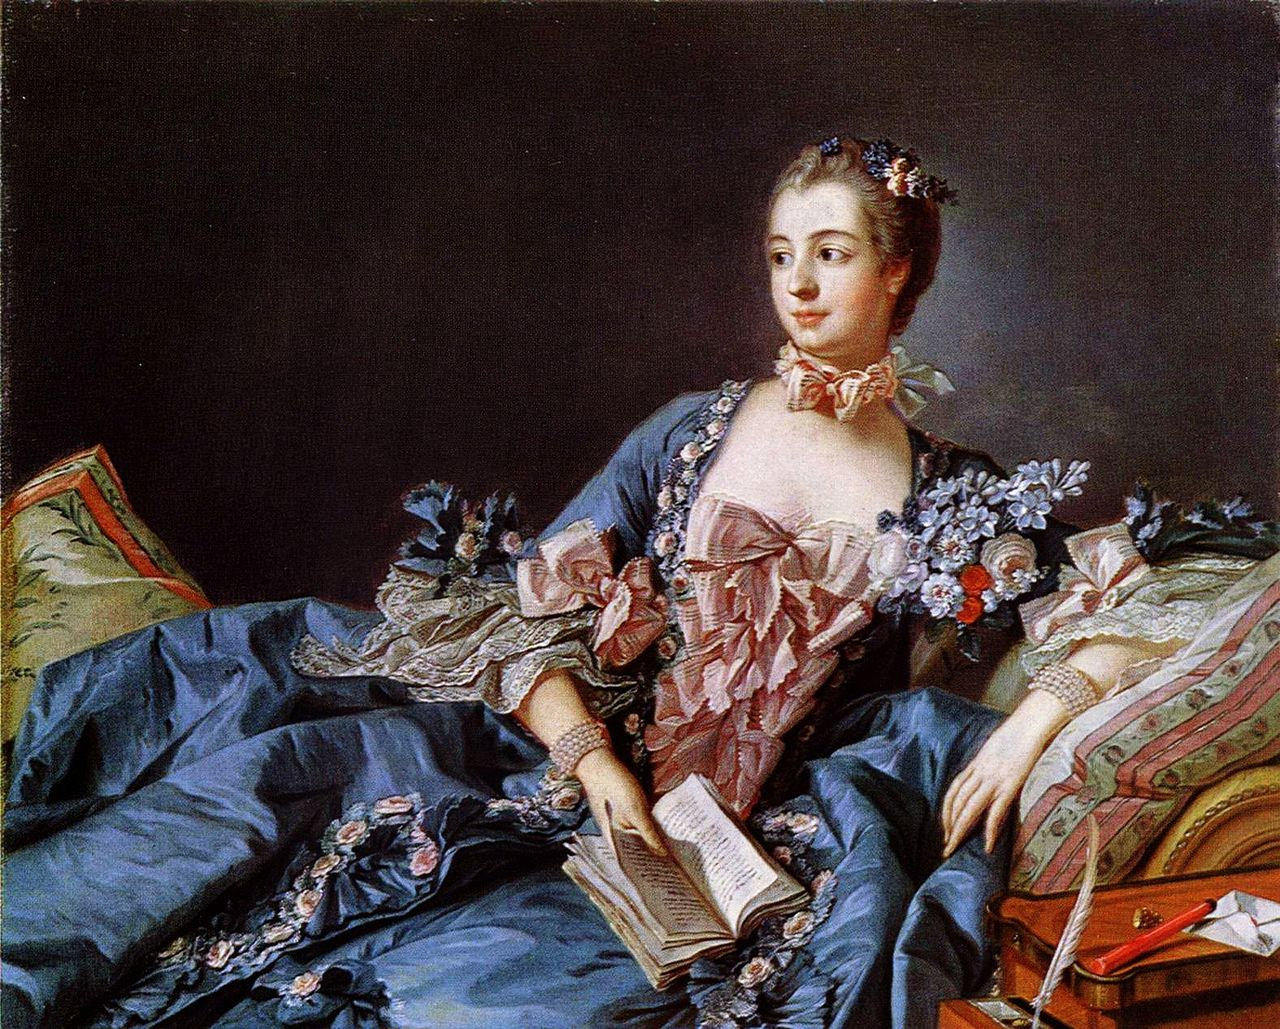
\includegraphics[height = 0.38\linewidth]{images/04_pompadour}
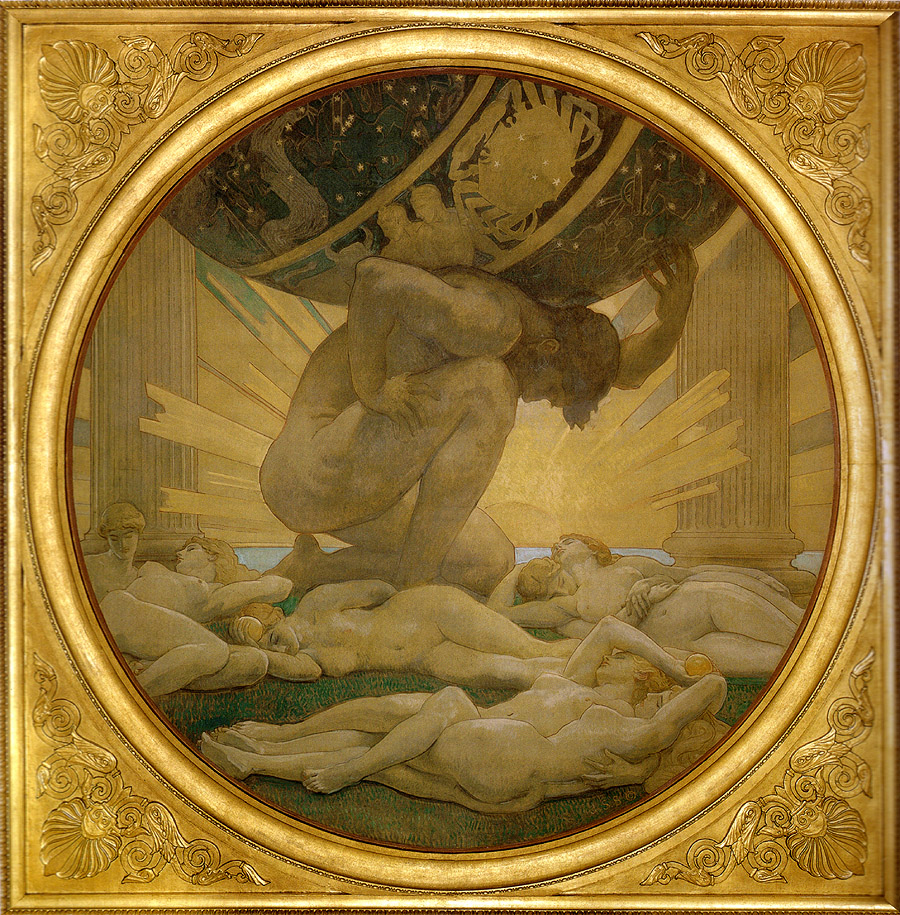
\includegraphics[height = 0.38\linewidth]{images/05_atlas}
\end{frame}

\begin{frame}{How should I choose?}
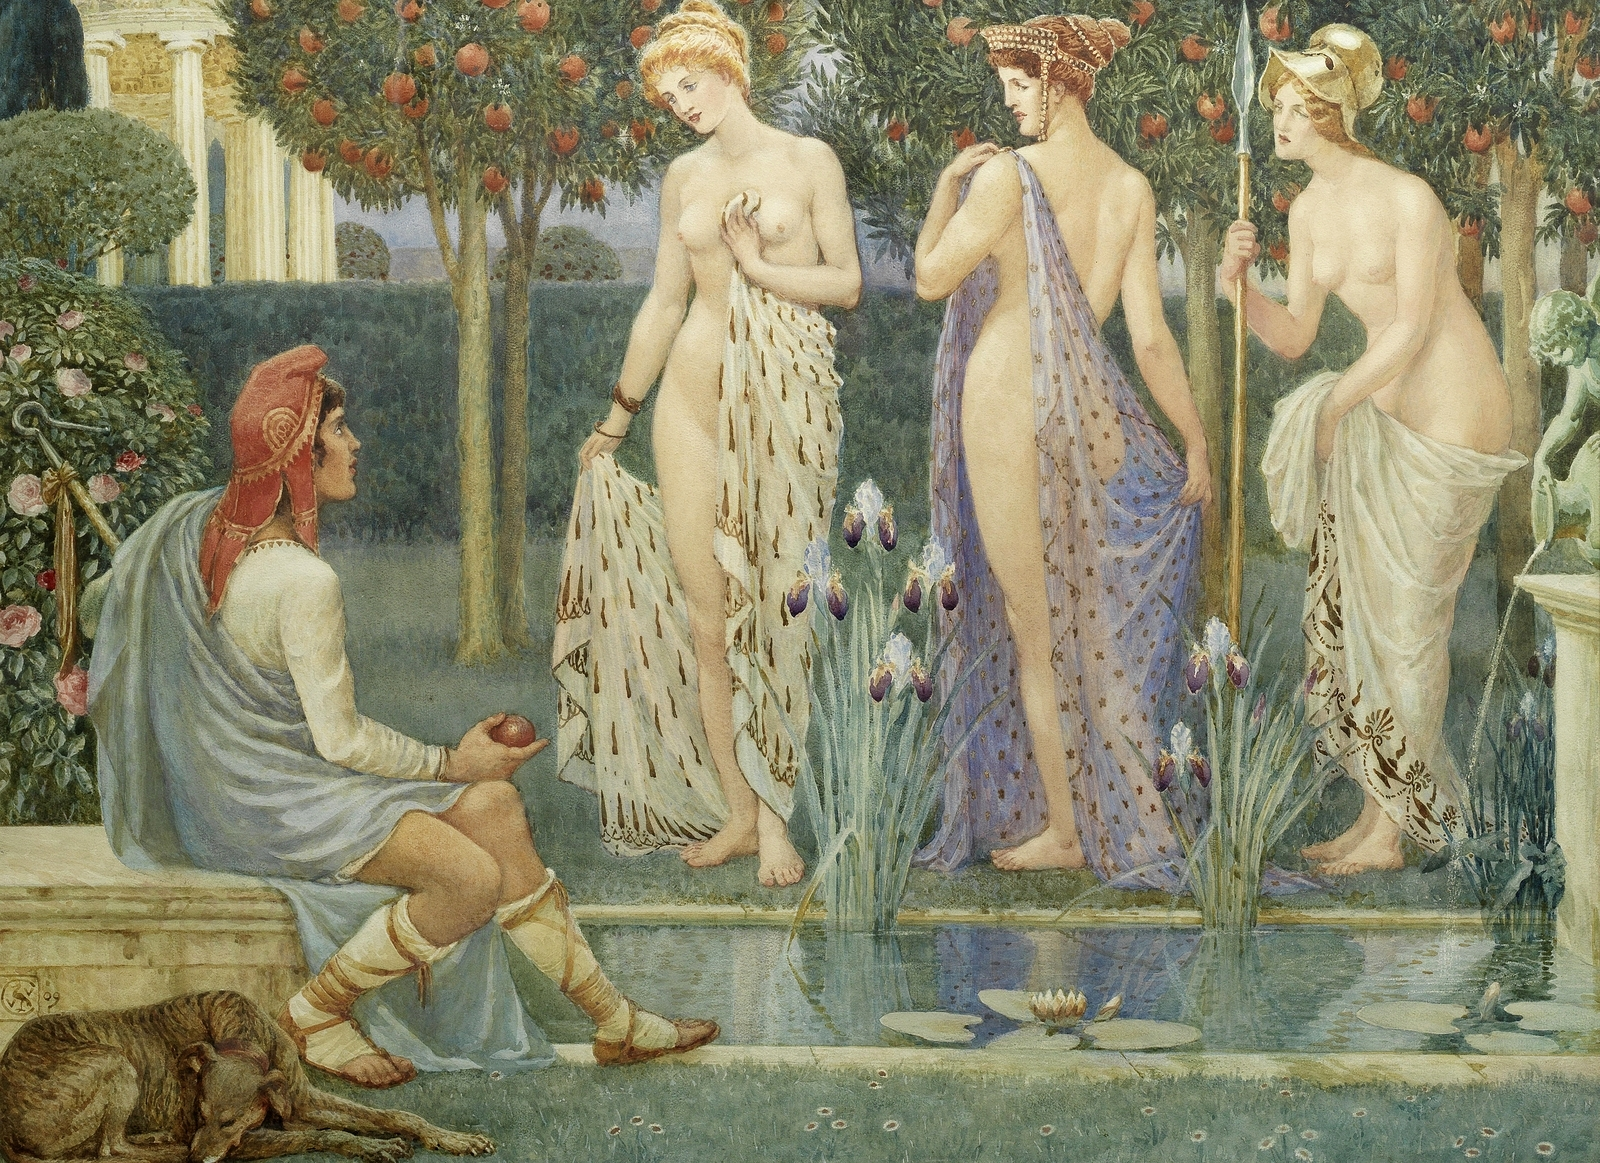
\includegraphics[width = \linewidth]{images/01_paris}\\
\small Walter Crane (1909) The Judgement of Paris
\end{frame}

\begin{frame}{THIS (122) vs. THAT (123) vs. THAT (124)}
\cite[144--145]{salimov10}\\
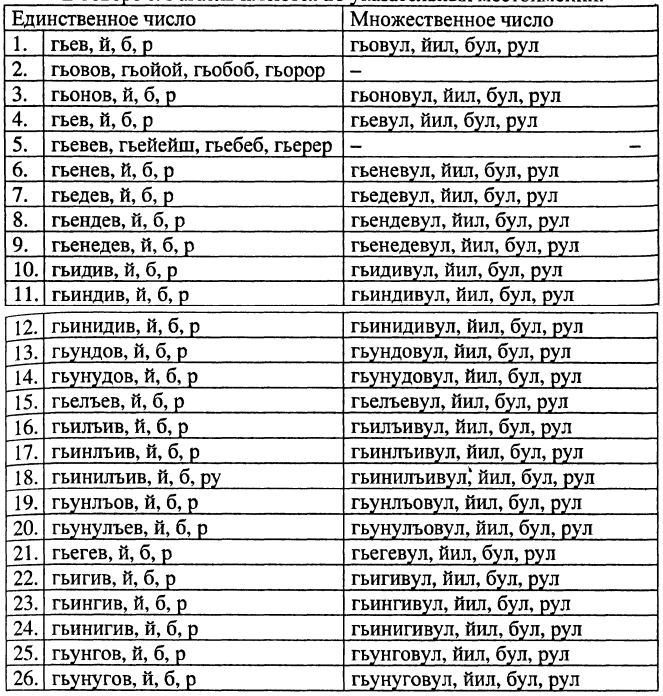
\includegraphics[width = 0.69\linewidth]{images/02_salimov}
\end{frame}

\begin{frame}{Searching for something that has already gone}
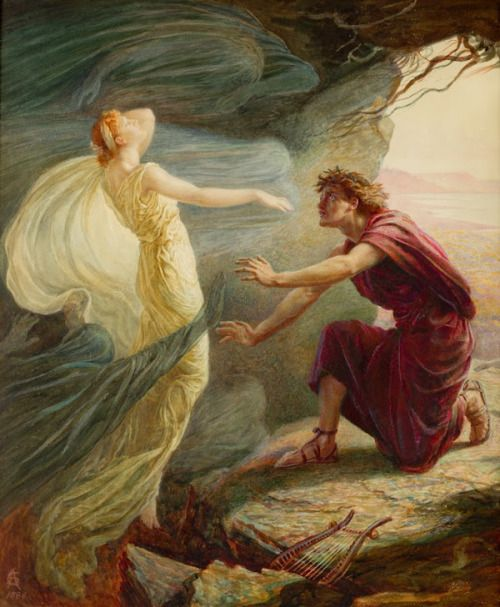
\includegraphics[width = 0.6\linewidth]{images/03_orpheus}\\
\small Catherine Adelaide Sparkes  Orpheus and Eurydice
\end{frame}

\begin{frame}{Searching for something that has already gone}
\begin{itemize}
\item SHEEP MILKING SHED (137), THRESHING-FLOOR (139), LOOM (512), WINNOW (613), FISHNET (1106) etc.
\item birds (HERON (175), HAWK (177), FALCON (178), SNOWCOCK (188)), animals (BADGER (198), ROE (208)), trees (LIME TREE (648), WILLOW (649), BARBERRY (662))
\item informant's memory...
\item[\dots] obscene lexicon (off-topic)
\end{itemize}
\end{frame}

\begin{frame}{Lets include this word!}
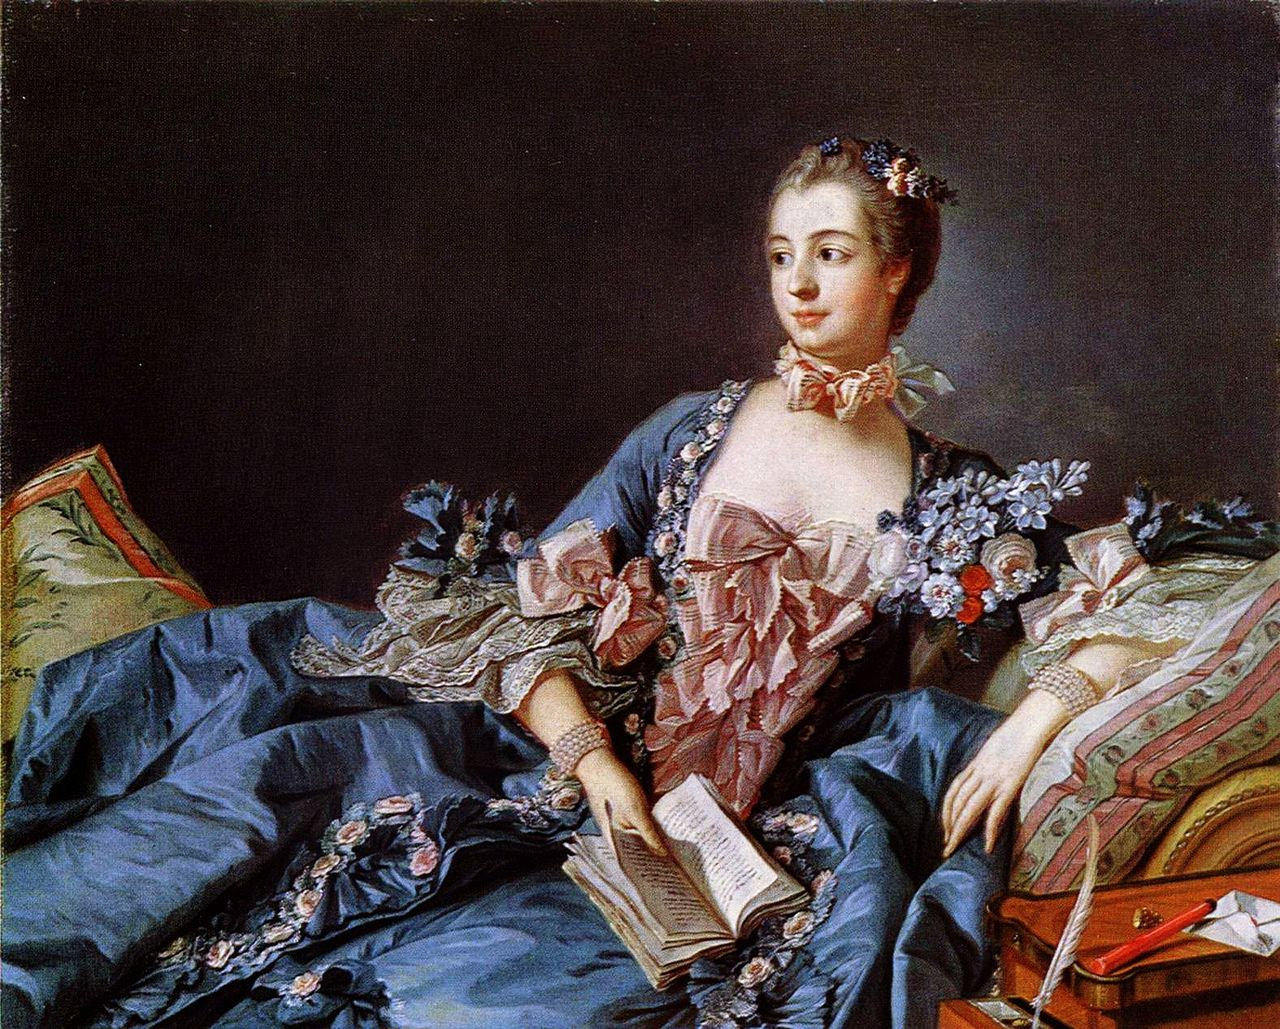
\includegraphics[width = 0.9\linewidth]{images/04_pompadour}\\
\small François Boucher (1759) Madame de Pompadour
\end{frame}

\begin{frame}{Audio recording}
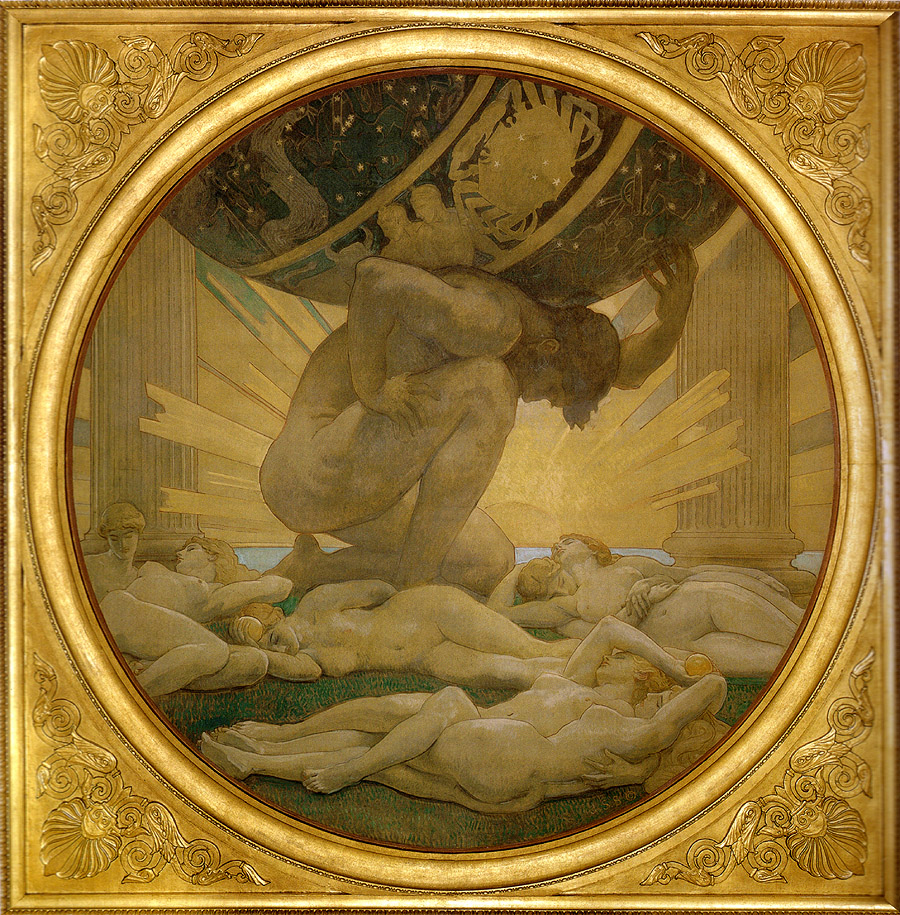
\includegraphics[width = 0.7\linewidth]{images/05_atlas}\\
\small John Singer Sargent (1925) Atlas and the Hesperides 
\end{frame}

\begin{frame}{Audio recording}
\begin{itemize}
\item informant was tired:\\
--- Последний рывок.\\
--- Что уже пора тебе сдохнуть?.. Последний рывок...
\item I was tired:\\
--- Ну-у-у, тут какой-то умник написал <<черемша>>, но мы пропустим наверное.\\
--- Черемша, он есть, но он у нас не растет.\\
--- А тмин?
\item Multiple times Informant continued session from the other room.
\item TV, chess, children...
\end{itemize}
\end{frame}

\begin{frame}{So our main problems are...}
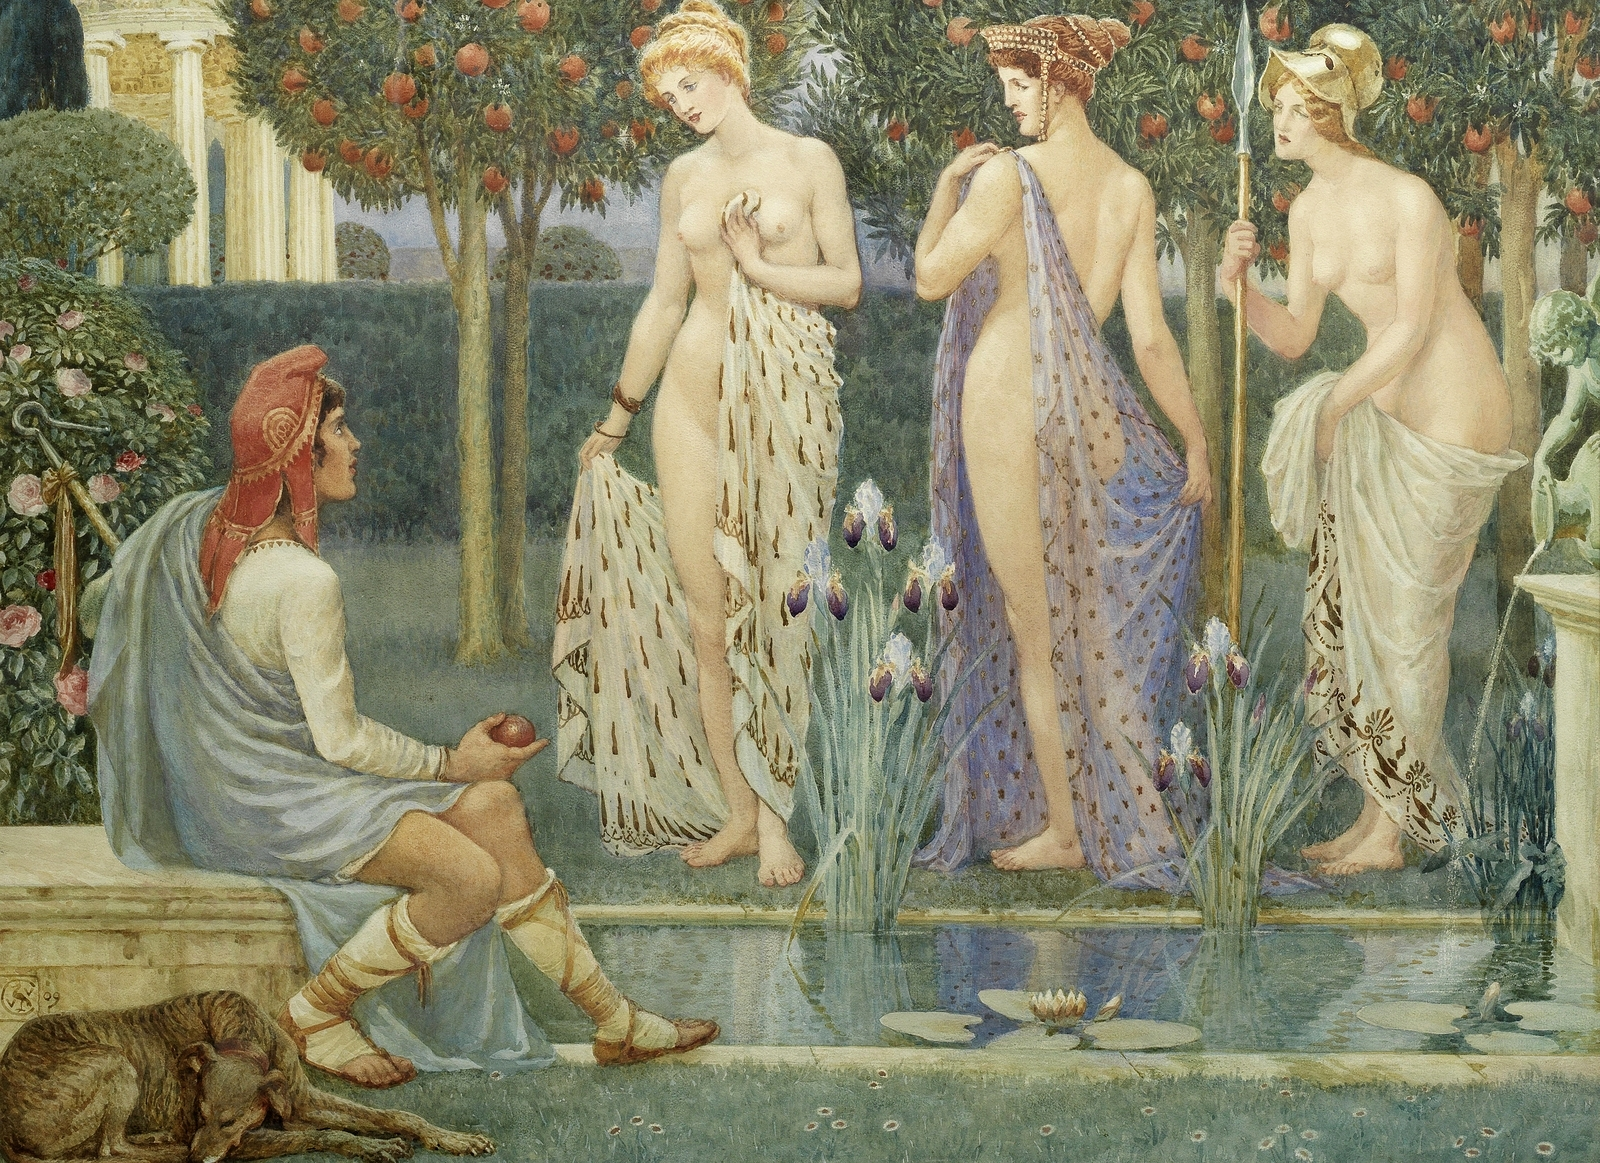
\includegraphics[height = 0.38\linewidth]{images/01_paris}
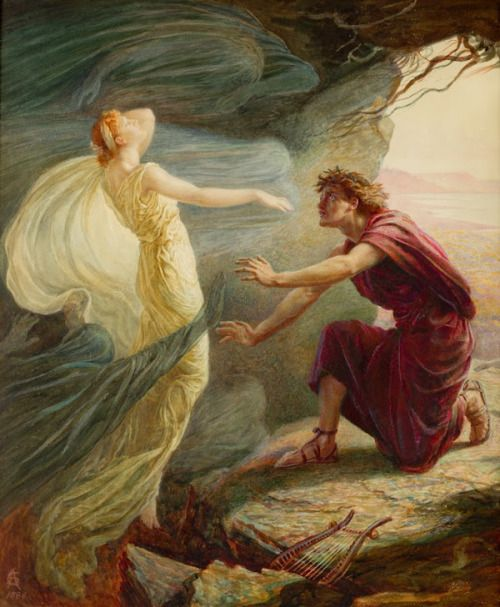
\includegraphics[height= 0.38\linewidth]{images/03_orpheus}\\
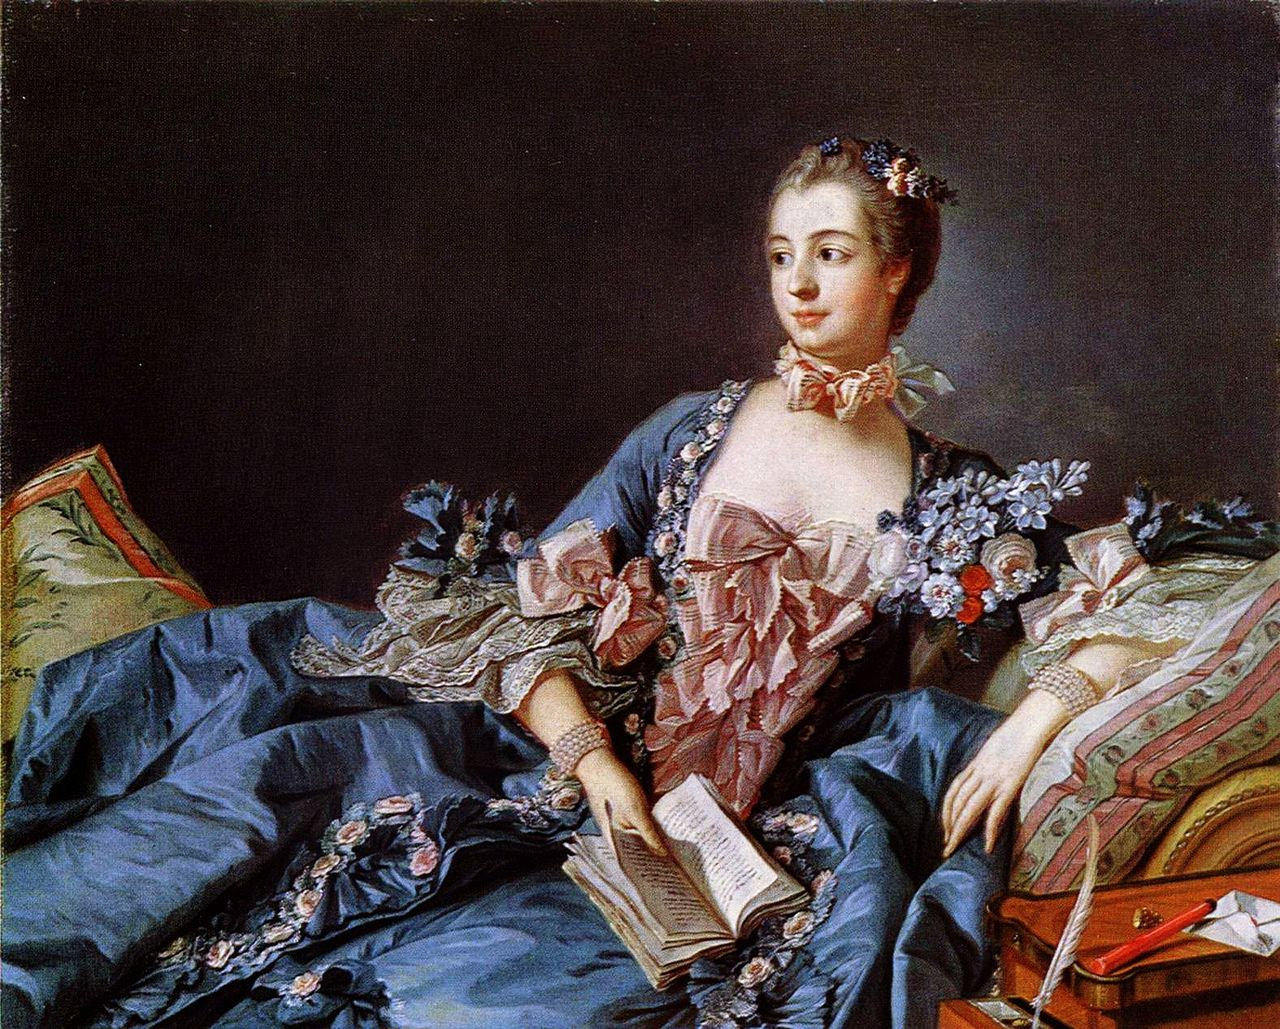
\includegraphics[height = 0.38\linewidth]{images/04_pompadour}
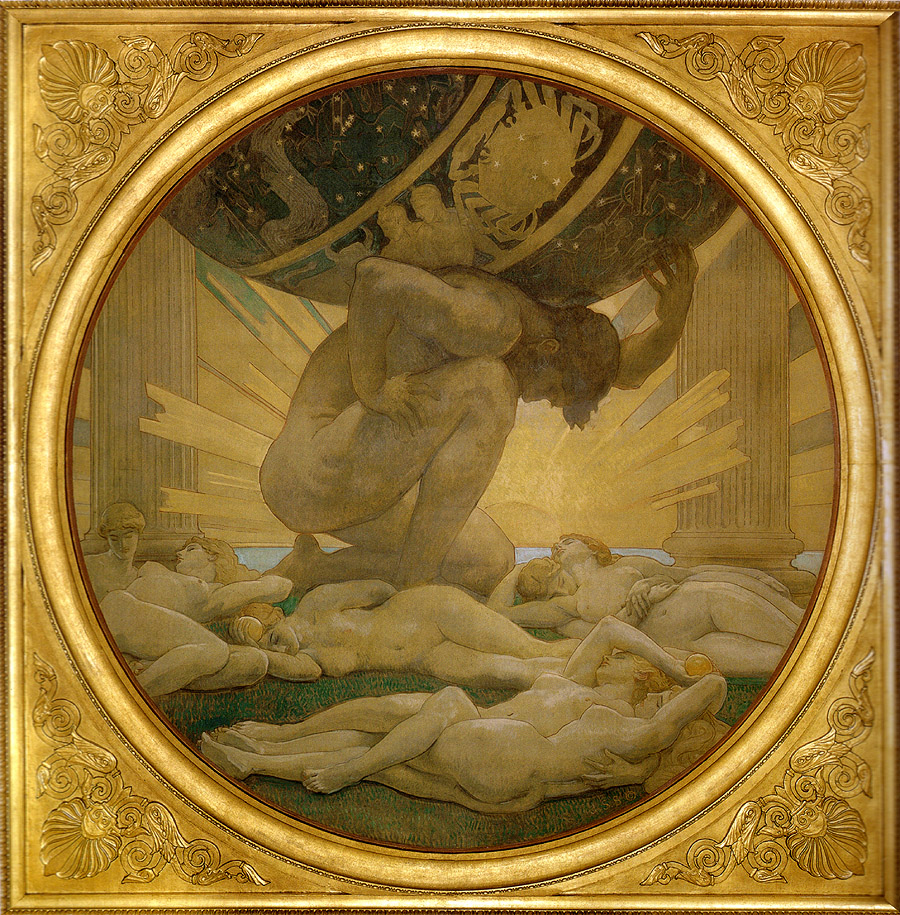
\includegraphics[height = 0.38\linewidth]{images/05_atlas}
\end{frame}

\begin{frame}{Language activism}
It is clear from our project that it is really hard to collect and analyse a lot of data. But what if some speakers will do it by themselves?
\begin{itemize}
\item our students and colleagues use VKontakte and Whatsup in their work
\item there are some local phone apps (Karata, Avar and Dargwa dictionary for Apple and Android)
\item \textbf{Wesay }and \textbf{Dictionary App Builder} by SIL are little bit old fashioned, but technology drastically improved!
\end{itemize}
\end{frame}

\framecard[colorblue]{{\color{colorwhite} \Large Send me a letter!\\
agricolamz@gmail.com}}

\begin{frame}{References}
\footnotesize
\bibliographystyle{config/chicago}
\bibliography{/home/agricolamz/work/bibliography.bib}
\vfill
{\tiny !еьлеб теаритс ен ашад}
\end{frame}

\end{document}